\documentclass[12pt,a4paper]{article}

\usepackage{fancyhdr}
\usepackage{graphicx}
\usepackage{placeins}
\usepackage{adjustbox}


\begin{document}

\pagestyle{fancy}
\fancyhf{}
\chead{Short summary report}

\begin{table}[t]
\centering
\caption {rnaQUAST metrics for assembled transcripts. In each row the best values are indicated with \textbf{bold}. For the transcript metrics (rows 4, 5, 6, 9, 13, 26, 27, 28) we highlighted the best \textbf{relative} values i.e. divided by the total number of transcripts in the corresponding assembly.}
\begin{adjustbox}{width=1\textwidth}
\small
\begin{tabular}{|l*{11}{|r}|}
\hline
\textbf{METRICS/TRANSCRIPTS}                            & \textbf{Trinity}       & \textbf{Trans-ABySS}   & \textbf{Oases}         & \textbf{SOAPdenovo-Trans} & \textbf{IDBA-Tran}     & \textbf{Bridger}       & \textbf{BinPacker}     & \textbf{Shannon}       & \textbf{rnaSPAdes}     & \textbf{SPAdes}        \\ \hline\hline
\multicolumn{11}{l}{\bf DATABASE METRICS}                                                 \\ \hline
Genes                                                   & 45792                  & 45792                  & 45792                  & 45792                  & 45792                  & 45792                  & 45792                  & 45792                  & 45792                  & 45792                  \\
Avg. number of exons per isoform                        & 6.262                  & 6.262                  & 6.262                  & 6.262                  & 6.262                  & 6.262                  & 6.262                  & 6.262                  & 6.262                  & 6.262                  \\ \hline
\multicolumn{11}{l}{\bf BASIC TRANSCRIPTS METRICS}                                        \\ \hline
Transcripts                                             & 63305                  & 135402                 & 243196                 & 101745                 & 55639                  & 54182                  & 2503                   & 53069                  & 76473                  & 44567                  \\
Transcripts $>$ 500 bp                                  & 30976                  & 47157                  & 100314                 & 20648                  & 23040                  & 27127                  & \textbf{2394}          & 26641                  & 28354                  & 20542                  \\
Transcripts $>$ 1000 bp                                 & 21804                  & 29719                  & 51832                  & 12603                  & 12294                  & 18266                  & \textbf{2037}          & 16915                  & 19367                  & 13099                  \\ \hline
\multicolumn{11}{l}{\bf ALIGNMENT METRICS}                                                \\ \hline
Aligned                                                 & 62410                  & 134605                 & 240548                 & 100986                 & \textbf{55367}         & 53312                  & 2489                   & 52618                  & 75637                  & 43715                  \\
Uniquely aligned                                        & 60559                  & 132078                 & 177880                 & 99816                  & 54884                  & 47785                  & 1590                   & 47310                  & 73243                  & 40569                  \\
Multiply aligned                                        & 310                    & 1098                   & 2382                   & 686                    & 289                    & 161                    & 5                      & 260                    & 306                    & 866                    \\
Unaligned                                               & 895                    & 797                    & 2648                   & 759                    & \textbf{272}           & 870                    & 14                     & 451                    & 836                    & 852                    \\ \hline
\multicolumn{11}{l}{\bf ALIGNMENT METRICS FOR NON-MISASSEMBLED TRANSCRIPTS}               \\ \hline
Avg. aligned fraction                                   & 0.993                  & 0.995                  & 0.891                  & 0.997                  & \textbf{0.998}         & 0.989                  & 0.946                  & 0.991                  & 0.989                  & 0.991                  \\
Avg. alignment length                                   & 1216.863               & 752.811                & 406.084                & 519.962                & 811.99                 & 1073.395               & \textbf{1972.809}      & 877.706                & 910.466                & 1089.264               \\
Avg. mismatches per transcript                          & 0.84                   & 0.316                  & 0.625                  & \textbf{0.163}         & 0.187                  & 0.913                  & 4.609                  & 0.802                  & 0.802                  & 0.706                  \\ \hline
\multicolumn{11}{l}{\bf ALIGNMENT METRICS FOR MISASSEMBLED (CHIMERIC) TRANSCRIPTS}          \\ \hline
Misassemblies                                           & 564                    & 612                    & 52668                  & \textbf{61}            & 41                     & 2643                   & 628                    & 1927                   & 1080                   & 570                    \\ \hline
\multicolumn{11}{l}{\bf ASSEMBLY COMPLETENESS (SENSITIVITY)}                              \\ \hline
Database coverage                                       & 0.208                  & \textbf{0.244}         & 0.024                  & 0.1                    & 0.096                  & 0.084                  & 0.011                  & 0.004                  & 0.111                  & 0.088                  \\
50\%-assembled genes                                    & 9280                   & \textbf{9765}          & 841                    & 4762                   & 4594                   & 4157                   & 811                    & 203                    & 5787                   & 4751                   \\
95\%-assembled genes                                    & 5323                   & \textbf{5721}          & 183                    & 2204                   & 967                    & 2100                   & 519                    & 71                     & 3185                   & 2629                   \\
50\%-covered genes                                      & 10171                  & \textbf{10804}         & 1206                   & 5293                   & 5313                   & 4421                   & 812                    & 259                    & 6064                   & 4919                   \\
95\%-covered genes                                      & 6275                   & \textbf{7145}          & 355                    & 2505                   & 1435                   & 2253                   & 526                    & 85                     & 3447                   & 2781                   \\
50\%-assembled isoforms                                 & 11611                  & \textbf{14134}         & 1064                   & 5063                   & 4846                   & 4637                   & 881                    & 206                    & 6289                   & 4955                   \\
95\%-assembled isoforms                                 & 6032                   & \textbf{6281}          & 183                    & 2244                   & 967                    & 2236                   & 554                    & 71                     & 3269                   & 2633                   \\
50\%-covered isoforms                                   & 12896                  & \textbf{16495}         & 1755                   & 5678                   & 5665                   & 4942                   & 883                    & 264                    & 6622                   & 5155                   \\
95\%-covered isoforms                                   & 7081                   & \textbf{8075}          & 360                    & 2548                   & 1436                   & 2397                   & 561                    & 85                     & 3544                   & 2785                   \\
Mean isoform coverage                                   & 0.649                  & 0.607                  & 0.246                  & 0.376                  & 0.434                  & 0.467                  & \textbf{0.808}         & 0.217                  & 0.509                  & 0.504                  \\
Mean isoform assembly                                   & 0.595                  & 0.539                  & 0.202                  & 0.343                  & 0.391                  & 0.444                  & \textbf{0.805}         & 0.195                  & 0.486                  & 0.487                  \\ \hline
\multicolumn{11}{l}{\bf GeneMarkS-T METRICS}                                              \\ \hline
Predicted genes                                         & 22949                  & 35418                  & \textbf{39050}         & 9941                   & 12246                  & 13562                  & 1924                   & 8919                   & 13269                  & 9048                   \\ \hline
\multicolumn{11}{l}{\bf ASSEMBLY SPECIFICITY}                                             \\ \hline
50\%-matched                                            & \textbf{35166}         & 68154                  & 24164                  & 22053                  & 17105                  & 13327                  & 1321                   & 912                    & 14553                  & 9643                   \\
95\%-matched                                            & \textbf{25522}         & 51506                  & 10182                  & 18742                  & 14889                  & 10017                  & 744                    & 469                    & 9593                   & 7028                   \\
Unannotated                                             & 20832                  & 54198                  & 149381                 & 71364                  & 33923                  & 30247                  & \textbf{100}           & 44108                  & 53812                  & 27678                  \\
Mean fraction of transcript matched                     & 0.554                  & 0.495                  & 0.122                  & 0.22                   & 0.311                  & 0.274                  & \textbf{0.78}          & 0.025                  & 0.193                  & 0.221                  \\ \hline
\end{tabular}
\end{adjustbox}
\end{table}

\FloatBarrier
\clearpage
\lfoot{generated by rnaQUAST}

\begin{figure}[t]
\centering
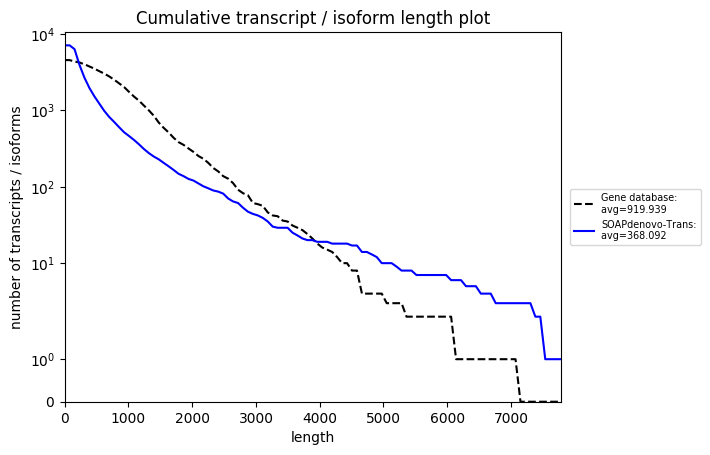
\includegraphics[width = \linewidth]{/mnt/dessertlocal/projects/transcriptome_assembly/review/evaluation/rna-quast/mmu/comparison_output/transcript_length.png}
\caption{Plot showing cumulative transcript length distribution. Each point represents the number of transcripts in the assembly with the corresponding length or longer; black dashed line corresponds to the database isoforms; the plot is given in logarithmic scale.}
\end{figure}
\FloatBarrier
\clearpage


\begin{figure}[t]
\centering
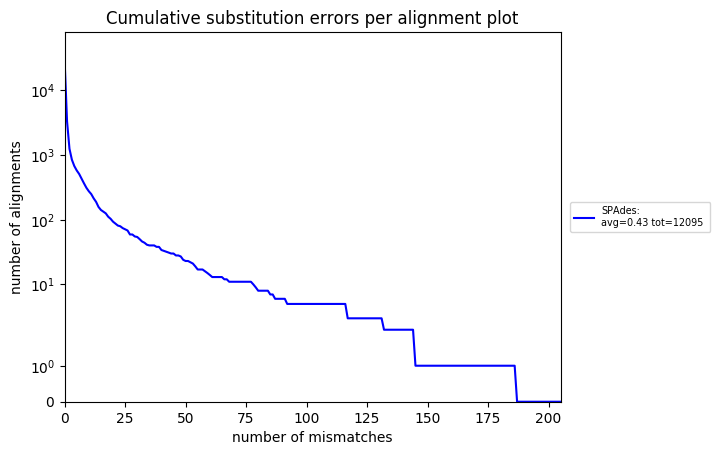
\includegraphics[width = \linewidth]{/mnt/dessertlocal/projects/transcriptome_assembly/review/evaluation/rna-quast/mmu/comparison_output/mismatch_rate.png}
\caption{Plot showing cumulative substitution errors per alignment distribution. Each point represents the number of alignments with the corresponding number of mismatches or greater; the plot is given in logarithmic scale.}
\end{figure}
\FloatBarrier
\clearpage


\begin{figure}[t]
\centering
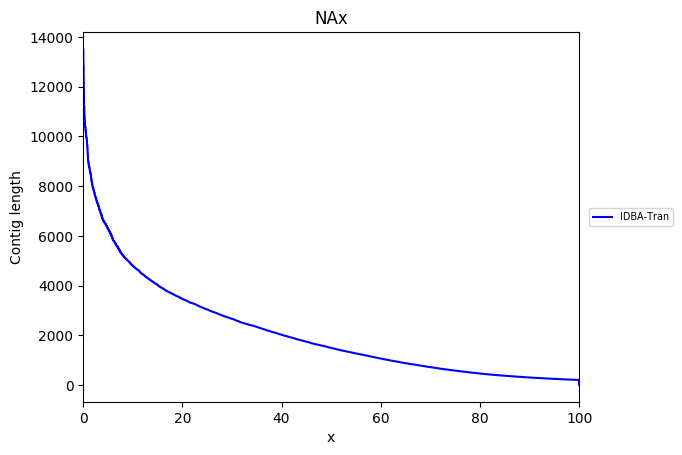
\includegraphics[width = \linewidth]{/mnt/dessertlocal/projects/transcriptome_assembly/review/evaluation/rna-quast/mmu/comparison_output/NAx.png}
\caption{Nx plot for transcripts. Nx is a maximal number $N$, such that the total length of all transcripts longer than $N$ bp is at least $x\%$ of the total length of all transcripts.}
\end{figure}
\FloatBarrier
\clearpage


\begin{figure}[t]
\centering
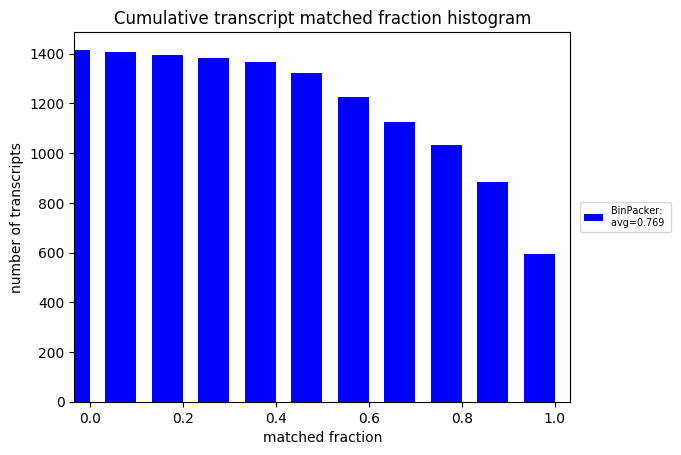
\includegraphics[width = \linewidth]{/mnt/dessertlocal/projects/transcriptome_assembly/review/evaluation/rna-quast/mmu/comparison_output/x-matched.png}
\caption{Plot showing cumulative transcript match histogram. Each bar represents the number of transcripts with matched fraction equal to or greater than the value on $x$ axis; transcript matched fraction is calculated as the number of its bases covering an isoform divided by the transcript length.}
\end{figure}
\FloatBarrier
\clearpage


\begin{figure}[t]
\centering
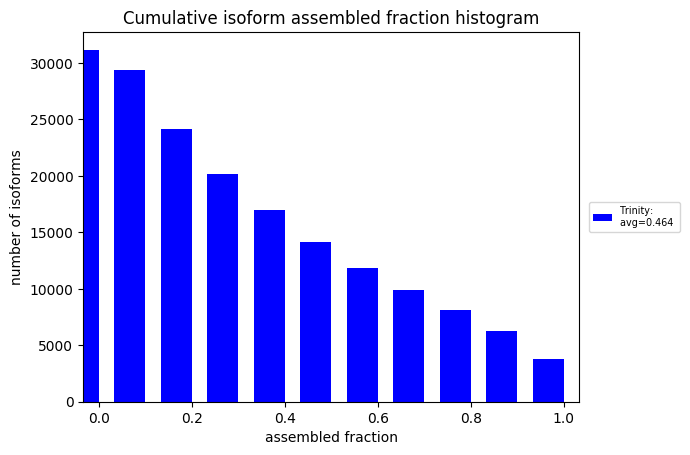
\includegraphics[width = \linewidth]{/mnt/dessertlocal/projects/transcriptome_assembly/review/evaluation/rna-quast/mmu/comparison_output/x-assembled.png}
\caption{Plot showing cumulative isoform assembly histogram. Each bar represents the number of isoforms with assembled fraction equal to or greater than the value on $x$ axis; isoform assembled fraction is calculated as the maximum number of captured by single assembled transcript bases divided by the total isoform length.}
\end{figure}
\FloatBarrier
\clearpage


\begin{figure}[t]
\centering
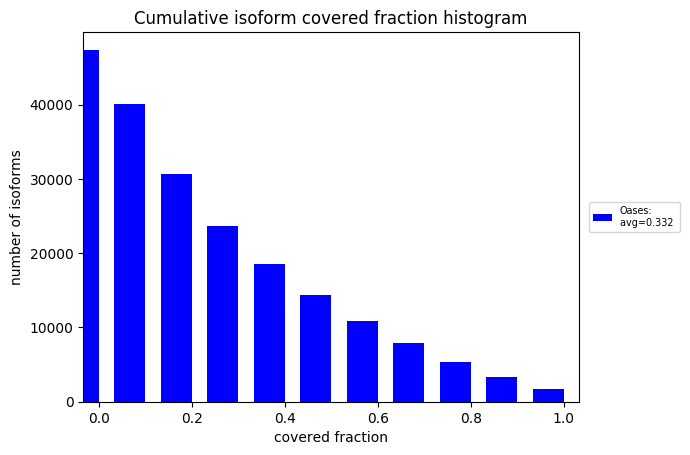
\includegraphics[width = \linewidth]{/mnt/dessertlocal/projects/transcriptome_assembly/review/evaluation/rna-quast/mmu/comparison_output/x-covered.png}
\caption{Plot showing cumulative isoform coverage histogram. Each bar represents the number of isoforms with covered fraction equal to or greater than the value on $x$ axis; isoform covered fraction is calculated as the number of covered bases (by all transcripts in the assembly) divided by the total isoform length.}
\end{figure}
\FloatBarrier
\clearpage


\end{document}
